\documentclass{article}
\usepackage{tikz}
\usepackage{amsmath}
\usetikzlibrary{angles,quotes}
\usetikzlibrary{decorations.pathmorphing,calc}
\begin{document}
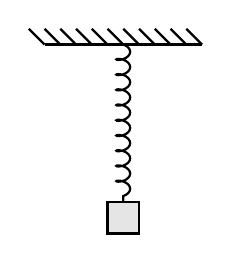
\begin{tikzpicture}[scale=1]
% Paramètres
\def\ressortL{2}   % longueur du ressort
\def\masseH{0.4}   % hauteur de la masse
\def\masseL{0.4}     % largeur de la masse
\def\x{0}
\def\dx{0.5}
\def\w{0.3}
\def\h{0.5}
\def\F{1}
\def\y{-2}
\def\dy{0}
% Support (plafond)
\draw[thick] (-1,0) -- (1,0);
\foreach \x in {-1,-0.8,...,1} {
  \draw[thick] (\x,0) -- (\x-0.2,0.2);
}
% Ressort vertical
\draw[
  thick,
  decorate,
  decoration={coil, segment length=5.5pt, amplitude=2.5pt}
] (0,0) -- (0,-\ressortL);
% Masse verticale
\draw[thick, fill=gray!20]
(-\masseL/2,-\ressortL-\masseH)
rectangle
(\masseL/2,-\ressortL);
\end{tikzpicture}
\end{document}